%! TEX program = pdflatex

\documentclass[oneside,solution]{seu-ml-assign}
\usepackage{CJK}
\usepackage{graphicx}
\usepackage{subfigure}
\usepackage{float}
\usepackage{setspace}
\usepackage{indentfirst}
\setlength{\parindent}{2em}
\renewcommand{\baselinestretch}{1.25}
\title{Homework}
\author{}
\studentID{}
\instructor{Zhengyang Liu}
\date{\today}
\duedate{July 17, 2022}
\assignno{1}
\semester{BIT --- 2022 Spring}
\mainproblem{Nash Equilibrium}

\begin{document}

\maketitle
%\startsolution[print]
\problem{Favourite Meal/Dish in School Canteen}
\begin{CJK}{UTF8}{gbsn}
东食堂二层的牛肉板面,学校少有的卖宽面条的地方,但对于不太能吃辣的我需要点微微微微辣的。
\end{CJK}

\problem{Equivalence of Nash Equilibrium's Definition}
%According to the consensus, the matrix notation should be the bold upper-case letter like $\mathbf{A}$ or $\bm{A}$, not $A$.
\subsection{Definition Clarification}
\\ \hspace*{\fill} \\
$\text{        }\quad\text{  }$ In this section, we modify formulas of the definition to make
preparations for further proof.

For \textbf{definition 1}, a pair of mixed strategies \((x,y)\) is Nash
Equilibrium iff neither of the player can increase their expected payoff
by deviating from the initial strategy while the other's unchanged.

Let \(R\) of size \(m\times n\) be the payoff matrix for the row player
and
\(\Delta_m=\{\mathbf{x}=\left(x_{1}, \ldots, x_{m}\right) \in \mathbb{R}^{m} \mid \sum_{i\in[m]}x_i=1,\)
\(x_i\geq 0 \}\)
be the set of all mixed strategies over \(m\) actions. When the strategy
\(y\) keeps constant, for \(\forall \mathbf{x^{'}} \in \Delta_m\), the
expected payoff for the row player \(\mathbf{x}^TR\mathbf{y}\) is always
greater than or equal to that of all other mixed strategies
\(\mathbf{x^{'}}R\mathbf{y}\), namely
\begin{equation}
\begin{aligned}
\mathbf{x}^TR\mathbf{y} \geq \mathbf{x}^{'T}R\mathbf{y},\; \forall \mathbf{x^{'}} \in \Delta_m
\end{aligned}
\label{equ:1}
\end{equation}

Define \(\mathbf{S}=R\mathbf{y} = \left\{s_1,s_2,\cdots,s_m\right\}\) to
simplify representations and rearrange equation Eq.~\eqref{equ:1}, i.e.
\(\mathbf{x}^{T}\mathbf{S}>\mathbf{x}^{'T}\mathbf{S}\),
\begin{equation}
\begin{aligned}
x_1s_1+x_2s_2+\cdots+x_ms_m&\geq x_1^{'}s_1+x_2^{'}s_2+\cdots+x_m^{'}s_m,\; \forall \mathbf{x^{'}} \in \Delta_m
\end{aligned}
\end{equation}

Let \(C\) stand for the payoff matrix for the column player, similarly,
for \(\forall \mathbf{y^{'}} \in \Delta_n\),
\begin{equation}
\begin{aligned}
\mathbf{x}^TC\mathbf{y} &\geq \mathbf{x}^{T}C\mathbf{y^{'}} \\
\mathbf{T}\mathbf{y} &\geq \mathbf{T}\mathbf{y^{'}}\\
y_1t_1+y_2t_2+\cdots+y_nt_n&
\geq y_1^{'}t_1+y_2^{'}t_2+\cdots+y_n^{'}t_n
\end{aligned}
\label{eq:2-3}
\end{equation}

where
\(\mathbf{T}=\mathbf{x}^{T}C = \left\{t_1,t_2,\cdots,t_n\right\}\).

For \textbf{definition 2}, a pair of strategies \((x,y)\) is Nash
Equilibrium iff each action in the support of \(\mathbf{x}\) (or
\(\mathbf{y}\)) is the best response to the other. When action \(x_i\)
is in favor of, namely the possibility for action \(i\) \(x_i\) is
greater than zero, the expected payoff of the pure strategy for action
\(i\) \(e_i^{T}R\mathbf{y}\) is better than all other pure strategies,
that is
\begin{equation}
    \begin{aligned}
        x_i>0 \Rightarrow \mathbf{e}_i^{T}R\mathbf{y}\geq \mathbf{e}_k^{T}R\mathbf{y}, \forall k \in [m]
    \end{aligned}
\end{equation}

Using notation \(\mathbf{S}\) as defined above, we can draw a conclusion
that
\begin{equation}
    \begin{aligned}
        x_i > 0 \Rightarrow s_i\geq s_k, \forall k \in [m]
    \end{aligned}
    \label{eq:2-5}
\end{equation}

Therefore, if \(x_i >0\) and \(x_k>0\), then \(s_i = s_k\), or it will
contradict Eq.~\eqref{eq:2-5}.

The same goes for the row player, for \(\forall k \in n\)
\begin{align}
y_j>0 &\Rightarrow \mathbf{x}^{T}C\mathbf{e}_{j}\geq \mathbf{x}^{T}C\mathbf{e}_k \label{eq:2-6}\\
y_j >0 &\Rightarrow t_j\geq t_k \label{eq:2-7}\\
y_i > 0,y_j>0 &\Rightarrow t_i=t_j \label{eq:2-8}
\end{align}


To sum up, definition 1 can be written in the form of Eq.~(\ref{eq:2-3}) and
definition 2 in the form of equation Eq.~\eqref{eq:2-6} and Eq.~\eqref{eq:2-7}, with its conclusion equation Eq.~\eqref{eq:2-8}.
\subsection{Proof of Equivalence}
\\ \hspace*{\fill} \\
$\text{        }\quad\text{  }$
In this section, using equations obtained previously, we aim to prove
equivalence from the perspective of sufficiency and necessity.
\paragraph{\(\text{a. Definition }1\Rightarrow \text{Definition } 2\)}
\begin{proof}
By contradiction. 

Assume that definition 2 does not hold. That is,
\begin{equation}
\begin{aligned}
\text{for }\mathbf{x} =\{x_1,x_2,\cdots,x_i,\cdots,x_k,\cdots,x_m\},\;x_i >0,
\exists k\in [m],\;\text{s.t. } s_i < s_k 
\end{aligned}
\end{equation}

As \(x_i>0\), \(x_is_i < x_i s_k\). It is obvious that
\( x_is_i+x_ks_k<x_is_k+x_ks_k=0+(x_i+x_k)s_k\).

Thus,
\(\exists \mathbf{x}^{'}=\{x_1^{},x_2\cdots,0,\cdots,x_i+x_k,\cdots,x_m\},\text{ s.t. }\mathbf{x}^{T}\mathbf{S}<\mathbf{x}^{'T}\mathbf{S}\).

However, this contradicts definition 1. 

Therefore, definition 1 is the sufficient condition for definition 2.
\end{proof}
\paragraph{\(\text{b. Definition }2\Rightarrow \text{Definition } 1\)}
\begin{proof}
    

Let \(\mathbf{\alpha}=\{a,b,\cdots,d\} \) be the set of all subscripts
that make \(x\) greater than \(0\), i.e., \(x_a>0,x_b>0\cdots,x_d>0\)
and \(x_a+x_b\cdots+x_d=1\). Then, there exists
\(\mathbf{\alpha}^{'}=\{o,p,\cdots,r\} \), which makes
\(x_o^{'}>0,x_p^{'}>0,\cdots,x_r^{'}>0\) and
\(x_o^{'}+x_p^{'}+\cdots+x_r^{'}=1\).

\paragraph{case 1: }\(\alpha^{'} \subseteq \alpha\)

Based on definition 2, \(s_a=s_b=\cdots=s_d=s_o=s_p=\cdots=s_r\).

Thus, \(x_1s_1+x_2s_2+\cdots+x_ms_m=(x_a+\cdots+x_c+x_d)s_a=s_a\).

Similarly, \(x_1^{'}s_1+x_2^{'}s_2+\cdots+x_m^{'}s_m=s_a\).

It can be inferred from above that
\(x_1s_1+x_2s_2+\cdots+x_ms_m=x_1^{'}s_1+x_2^{'}s_2+\cdots+x_m^{'}s_m\),
which satisfies definition 1.

\paragraph{case 2: }\(\alpha^{'}\not\subseteq \alpha\)

\(\exist x_p=0 ,x_p^{'} > 0\), according to definition 2 in equation Eq.~\eqref{eq:2-5}, for \(x_a>0,s_a\geq s_p\).

Thus,
\(x_1^{'}s_1+x_2^{'}s_2+\cdots+x_m^{'}s_m=(x_o^{'}+\cdots+x_r^{'})s_a+x_p^{'}s_p\leq(x_o^{'}+\cdots+x_r^{'}+x_p^{'})s_a=s_a\).

As \(x_1s_1+x_2s_2+\cdots+x_ms_m=(x_a+\cdots+x_c+x_d)s_a=s_a\),
\(\mathbf{x}^{T}\mathbf{S}\geq\mathbf{x}^{'T}\mathbf{S}\), which
satisfies definition 1.


Combining case 1 and case 2, definition 2 is the necessary condition for
definition 1.
\end{proof}
Hence, two definitions are equivalent.

\problem{Proof of Symmetric Nash Equilibrium}
We can solve the problem using \textbf{Brouwer's Fixed Point Theorem}:
let \(D\) be a convex and compact subset of \(\mathbb{R}^n\). If a
function \(f:\;D\rightarrow D\) is continuous, then exists \(x\in D\)
such that \(f(x) = x\). Firstly, we will construct a function that
satisfies the theorem's requirement. Then, we will prove that any fixed
point of function \(f\) is an Nash Equilibrium of the game.
\subsection{Construction of Function $f$}
\\ \hspace*{\fill} \\
$\text{        }\quad\text{  }$
For Nash Equilibrium, set \(f:\Delta\rightarrow\Delta\), where
\(\Delta\) is the set containing mixed strategies of the row player
(referred as player 1 in the following part) and the column player
(referred as player 2 in the following part). Thus, \(\Delta\) can be
described as \([\mathbf{x},\mathbf{x}]\), where \(x\in\Delta_m\) as
defined in Problem 2.

The expected payoff for player 1 and 2, similar to Problem 2, is as
follows:
\begin{equation}
\begin{aligned}
u(\mathbf{x}_1)&=\mathbf{x}_1^TR\mathbf{x_2}\\
u(\mathbf{x}_2)=\mathbf{x}_1^TC\mathbf{x}_2=\mathbf{x}_1^TR^T\mathbf{x}_2&=(\mathbf{x}_1^TR^T\mathbf{x}_2)^T=\mathbf{x}_2^TR\mathbf{x}_1
\end{aligned}
\end{equation}
Define a gain function
\(G_{p,s_p}=\max(u_p(s_p;\mathbf{x}_{-p})-u_p(\mathbf{x}),0)\) to
describe the utility player \(p\) can increase using pure strategy
\(s_i\), when the other's mixed strategy is fixed,

\begin{equation}
\begin{aligned}
G_{1,s_1}=\max(\mathbf{e}_{s_1}^TR\mathbf{x}_2-\mathbf{x}_1^TR\mathbf{x_2},0)\\
G_{2,s_2}=\max(\mathbf{e}_{s_2}^TR\mathbf{x_1}-\mathbf{x}_2^TR\mathbf{x_1},0)
\end{aligned}
\label{eq:3-2}
\end{equation}

Let \(\mathbf{y}=f(\mathbf{x})\), where

\begin{equation}
    y_{p,s_p}=\frac{x_{p,s_p}+G_{p,s_p}(\mathbf{x})}{1+\sum_{s^{'}_p\in S_P}G_{p,s^{'}_p(\mathbf{X})}}
\end{equation}

If \(\mathbf{x}_1=\mathbf{x}_2\), according to equation Eq.~\eqref{eq:3-2}, then
\(G_{1,s_1}=G_{2,s_2}\). Thus, \(\mathbf{y}_1=\mathbf{y}_2\). For
\(\Delta=[\mathbf{x},\mathbf{x}]\), \(f\) satisfies the mapping
\([\mathbf{x},\mathbf{x}]\rightarrow[\mathbf{y},\mathbf{y}]\). For each
player \(\sum y_{p,s_p} =1\) and \(y_{p,s_p}\geq 0\), meaning that
\([\mathbf{y},\mathbf{y}]\in \Delta\). Therefore, the mapping can be
turned into \(\Delta \rightarrow \Delta\). Moreover, \(f\) is
continuous. According to Brouwer's Fixed Point Theorem, there exists a
\(\mathbf{X}=[\mathbf{x},\mathbf{x}] \in \Delta\) such that
\(f(\mathbf{\mathbf{X}})=\mathbf{X}\).
\subsection{Proof of any Fixed Point being an NE of the
Game}
\\ \hspace*{\fill} \\
$\text{        }\quad\text{  }$
To show a fixed point \([\mathbf{x},\mathbf{x}]\) is the symmetric Nash
Equilibrium of the game, we only need to prove that
\(G_{p,s_p}(\mathbf{x})=0,\forall p\in[2]\).
\begin{proof}

By contradiction.

Assume that \(G_{p,s_p}(\mathbf{x})=0\) does not hold. That is, there
exists \(p\in[2],s_p\) such that \(G_{p,s_p}>0\).

As \([\mathbf{x},\mathbf{x}]\) is a fixed point, we can infer that
\(x_{p,s_p}>0\). Otherwise, if \(x_{p,s_p}=0\), then
\(y_{p,s_p}>0 \neq x_{p,s_p}\), which breaks the premise that
\([\mathbf{x},\mathbf{x}]\) is a fixed point.

For player \(p\), the utility \(u_p(\mathbf{x})\) equals the sum of
\(x_{p,s_p}\cdot u_p(s_p;\mathbf{x}_{-p}),\forall s\in S_p\). If
\(G_{p,s_p}>0\), then according to the definition of the gain function,
\(u_p(s_p;\mathbf{x}_{-p})>u_p(\mathbf{x})\). Moreover, as mentioned
above, \(x_{p,s_p}>0\). Hence, to make the equation
\(u_p(\mathbf{x})=\sum_{s\in S_p}x_{p,s_p}\cdot u_p(s_p;\mathbf{x}_{-p})\) hold,
there exists some other pure strategy \(s_p^{'}\) such that
\(x_{p,s_p^{'}}>0\) and \(u_p(s_p;\mathbf{x}_{-p})>u_p(\mathbf{x})\). In
this case, \(G_{p,s_p}<0\) and \(y_{p,s_p^{'}}<x_{p,s_p^{'}}\). However,
this contradicts the fact that \([\mathbf{x},\mathbf{x}]\) is a fixed
point.

Hence, there exists \(G_{p,s_p}(\mathbf{x})=0,\forall p\in[2]\) and any
symmetric game \((R,C)\) where \(R=C^T\) has a symmetric Nash
Equilibrium \([\mathbf{x},\mathbf{x}]\).
\end{proof}
\problem{Proof of Sperner's Lemma}
\subsection{Proof by double-counting}


\begin{proof}
We can prove the lemma by counting the number of yellow-blue edges from
two different perspectives.

\paragraph{a. Counting By Color} 
\\ \hspace*{\fill} \\
$\text{        }\quad\text{  }$
Assume that there are \(a\) triangles colored
by all the three colors and \(b\) triangles colored by yellow and blue,
as is shown in Figure \ref{fig:1}.
\begin{figure}[H]
  \centering
  \subfigure[One Yellow-blue Edge]{
    \label{fig:subfig:onefunction} 
    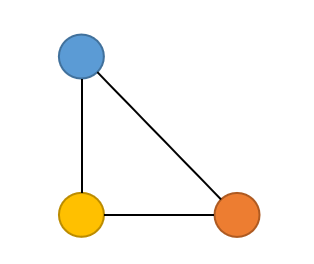
\includegraphics[scale=0.9]{Figure/g1a.png}}
  \hspace{0.5in} % 两图片之间的距离
  \subfigure[Two Yellow-blue Edges]{
    \label{fig:subfig:twofunction} 
    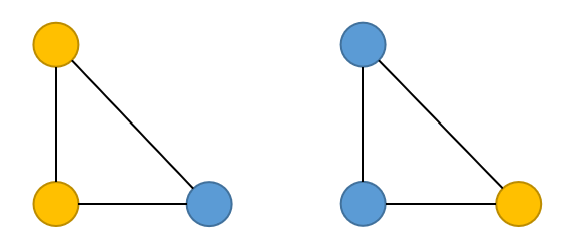
\includegraphics[scale=0.9]{Figure/g1b.png}}
  \caption{Counting by color}
  \label{fig:1} 
\end{figure}


Thus, the number of yellow-blue edges all triangles contain is \(a+2b\).

\paragraph{b. Counting by position}
\\ \hspace*{\fill} \\
$\text{        }\quad\text{  }$
As can be seen in the figure of the problem,
triangles inside the square share edges so that all yellow-blue edges
can be counted twice in the last section. Meanwhile, when yellow-blue
edges are the boundary of the square, they are counted only once. Assume
there are \(c\) internal edges and \(d\) boundary edges, the number of
yellow-blue edges all triangles contain can be double-counted as
\(2c+d\).

According to the way by which we are supposed to color the boundary,
there are no yellow node on the top and right boundary, no blue on the
left. Thus, yellow-blue edges can only appear at the bottom of the
square. Moreover, the lower left node are supposed to be yellow, the
lower right node blue. Therefore, there must be an odd number of
yellow-blue edges on the bottom boundary, meaning that \(d\) is an odd
number.

As two ways of counting are equivalent, \(a+2b=2c+d\). As \(d\) is an
odd number, \(a\) is also an odd number, which proves the existence of a
tri-chromatic triangle.
\end{proof}

\subsection{Proof by path-following}
\begin{proof}
Firstly, we will define directed edges, as is shown in Figure \ref{fig:2}.
The path start from the center of a triangle to the center of another.
It can cross the adjacent edge of two triangles only when the edge is
yellow-red with red on our left hand.

\begin{figure}[H]
\centering
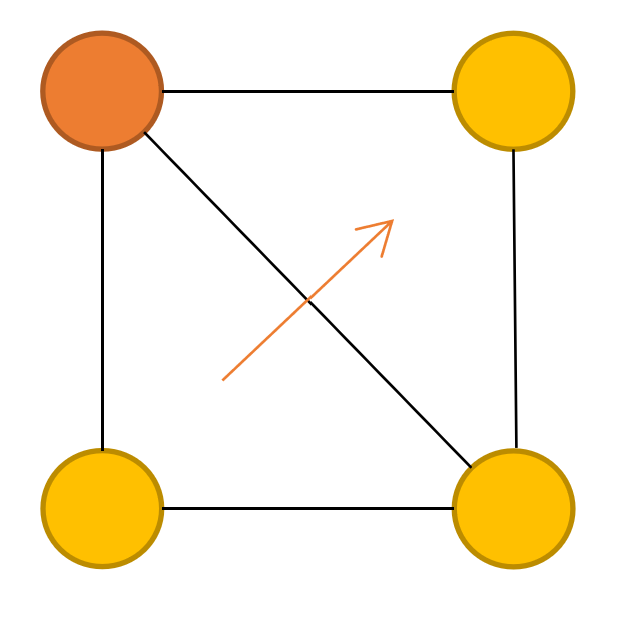
\includegraphics[width=3cm]{Figure/g2.png}
\caption{Definition of Directed Edges}
\label{fig:2}
\end{figure}

Then, for convenience, we introduce an outer boundary for the square in
Figure \ref{gra:3}. It is obvious that this way of adding an outer boundary
does not result in more tri-chromatic triangles. We set the initial
source node in the bottom-left triangle, as is marked in the following
figure. Following the rule of directed path as mentioned above, we
wander around the square.

\begin{figure}[H]
\centering
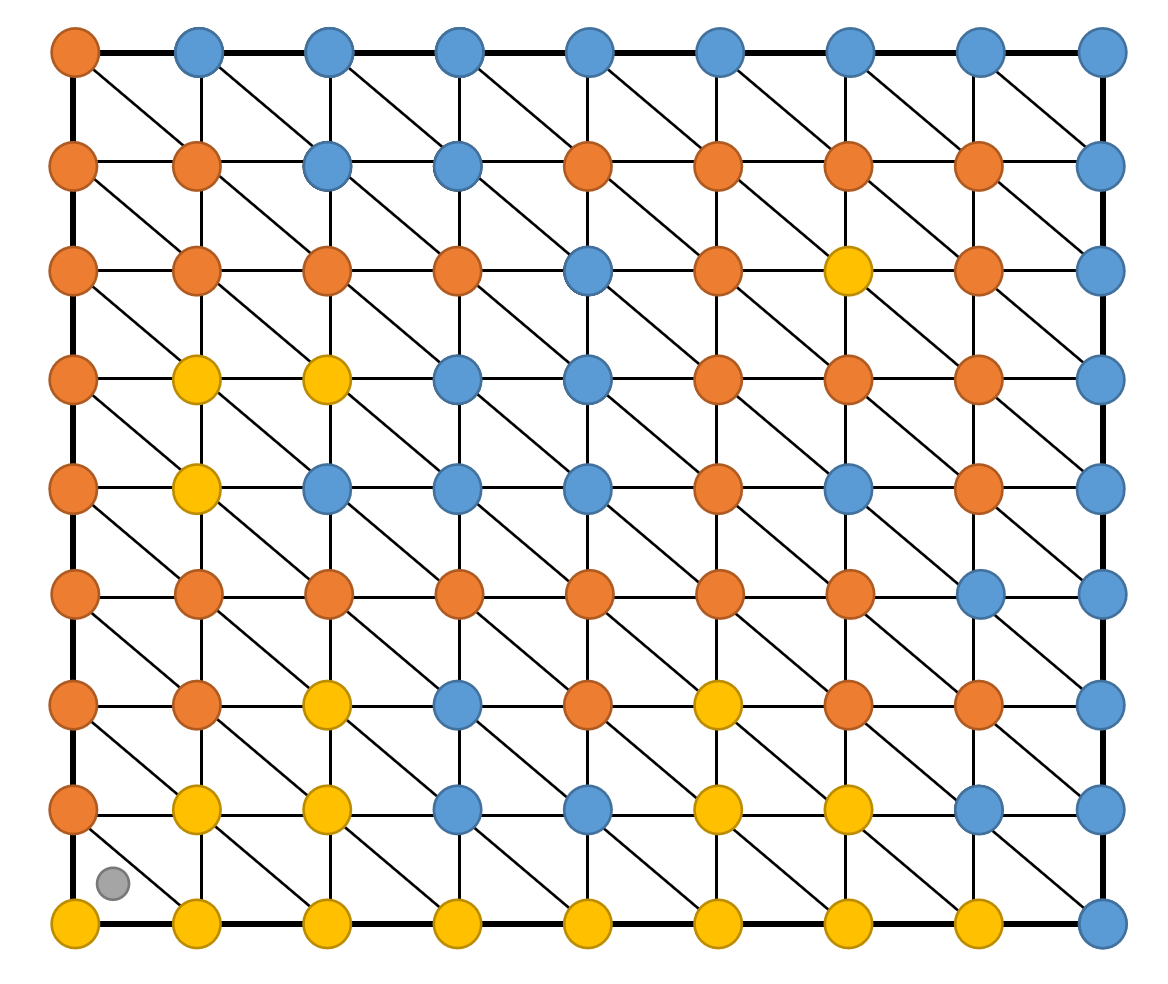
\includegraphics[width=7cm]{Figure/g3.png}
\caption{Introduction of an Outer Boundary}
\label{gra:3}
\end{figure}

As we can only cross yellow-red edges with red on left hand, yet there's
only one yellow-red edge with red on right hand in the outer boundary,
as a result, the walk cannot exit the square. Neither could it loop
inside. There will be a loop when there's a closed red square, according
to Figure \ref{fig:4}. But based on the rule we've designed, this could not
happen. Hence, the path must stop somewhere inside the square.
\begin{figure}[H]
  \centering
  \subfigure[Loop]{
    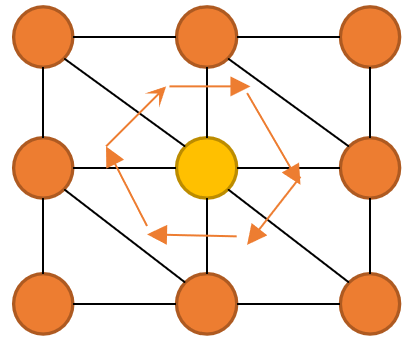
\includegraphics[scale=0.6]{Figure/g5a.png}}
  \hspace{0.5in} % 两图片之间的距离
  \subfigure[No Loop]{
    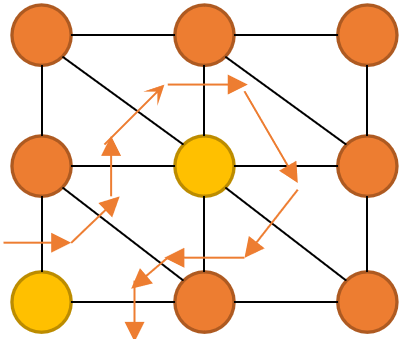
\includegraphics[scale=0.6]{Figure/g5b.png}}
  \caption{Loop Conditions}
  \label{fig:4} 
\end{figure}

The path will stop only in a triangle colored by all the three colors
(see Figure \ref{fig:5}). This proves the existence of a tri-chromatic
triangle.
\begin{figure}[H]
\centering
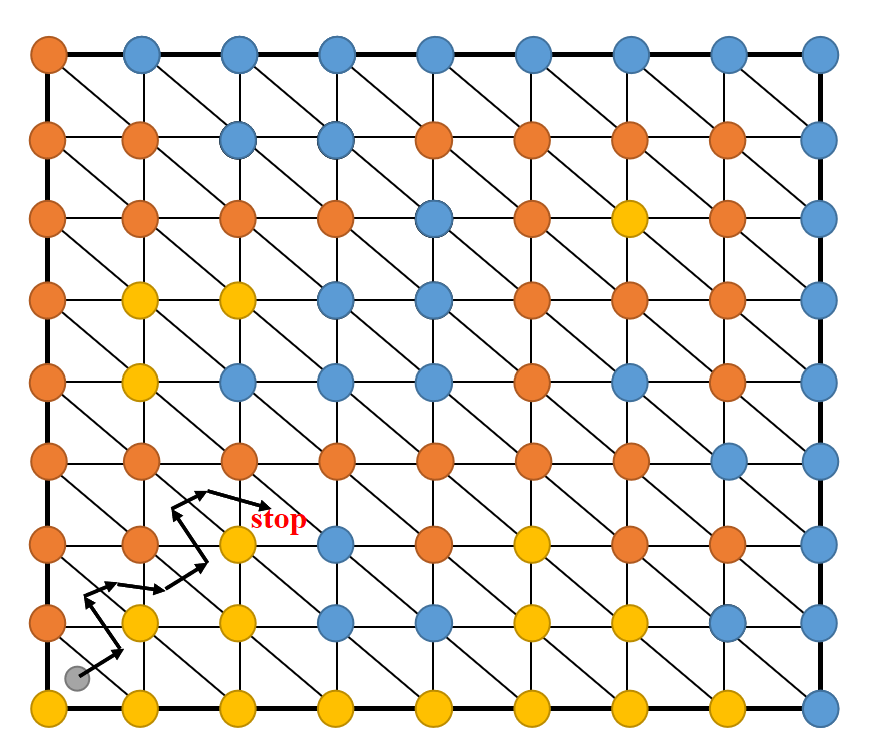
\includegraphics[width=7cm]{Figure/g5.png}
\caption{Stop Conditions}
\label{fig:5}
\end{figure}

\end{proof}


\end{document}
